\section{Human Evaluation and Interviews}\label{appx:user}
\subsection{Instructions and Trial Order}\label{appx:user_scenarios}\label{appx:user_assignment}
Participants receive task goals, object categories, and available actions, then answer queries through a tablet displaying camera views (Fig.~\ref{fig:app_human_tablet}). Ours requests Boolean state confirmations, potentially several per episode. KnowNo requests one action choice per trigger and permits manual entry. Each participant completes two trials per method and domain.

Let A denote Ours and B denote KnowNo. P1 and P5 complete Sort before Harvest with method order AABB. P2 completes the domains in reverse order with ABAB. P3 follows Sort then Harvest with BBAA, and P4 follows the reverse domain order with BABA. Each method sequence applies to both domains.

\begin{figure}[t]
\centering
\captionsetup[subfigure]{font=small,skip=2pt}
\begin{subfigure}[t]{0.485\linewidth}
\centering
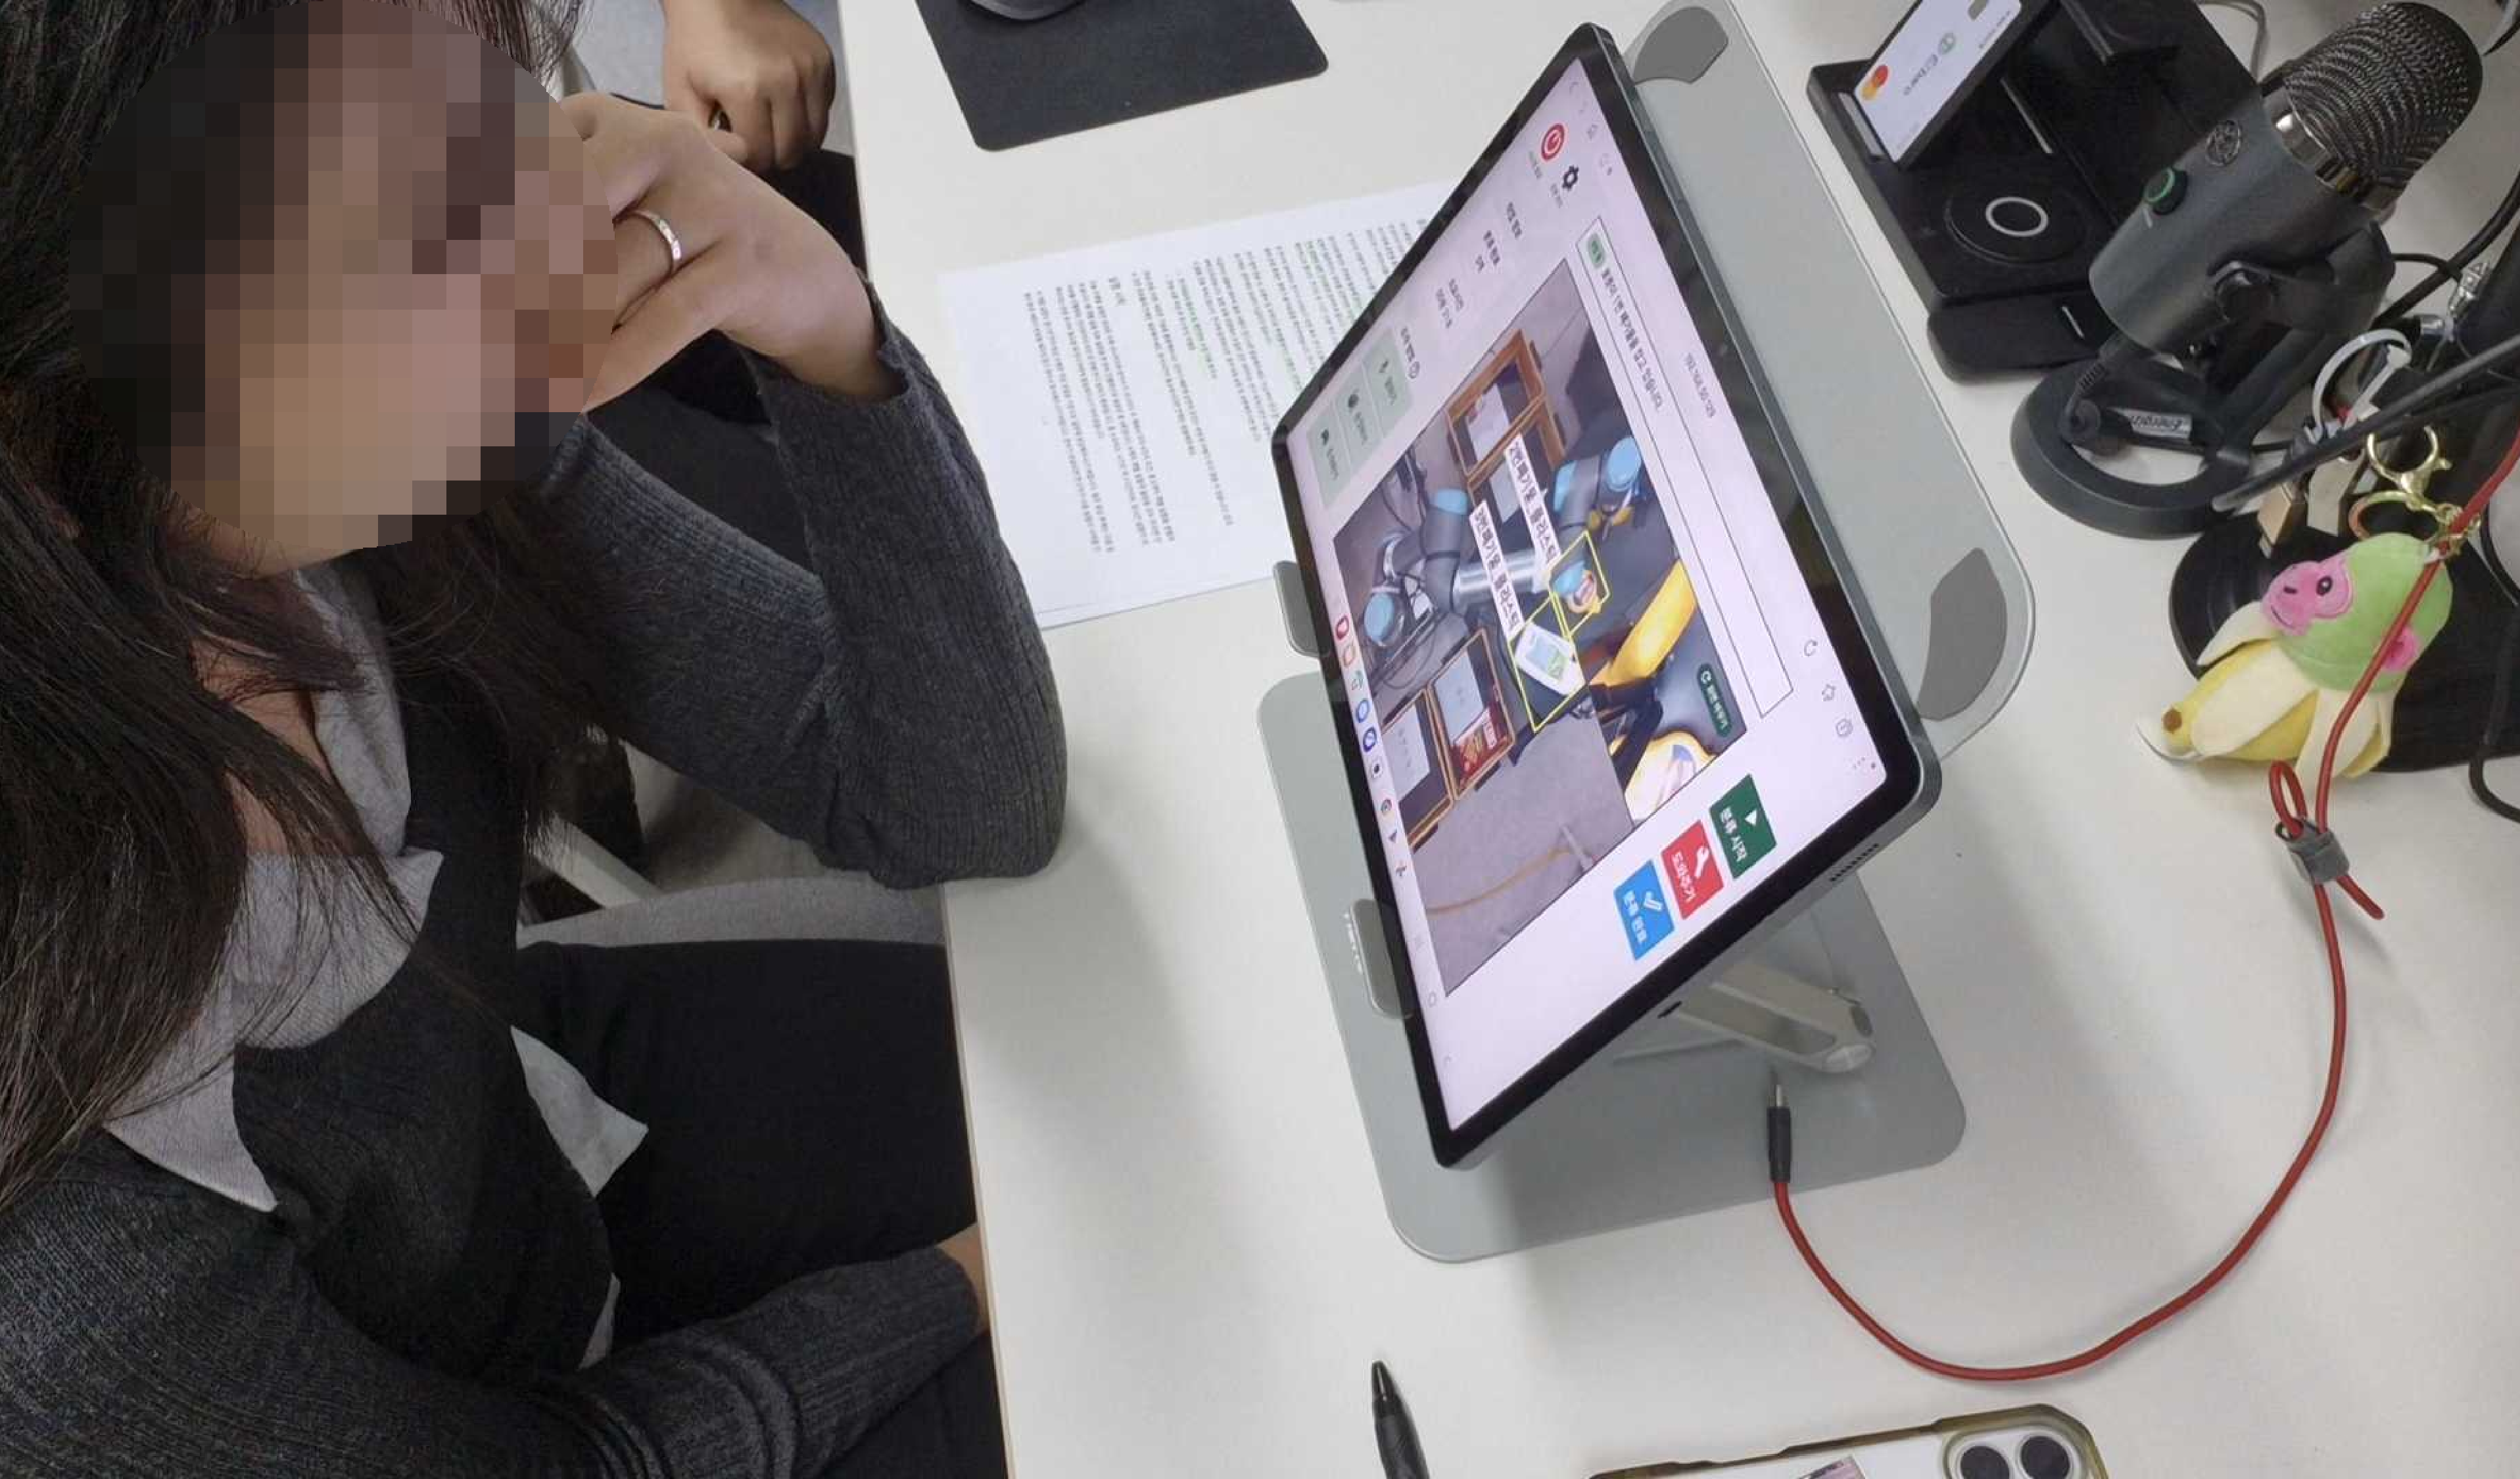
\includegraphics[width=\linewidth]{figures/10_APPX/p3_test.pdf}
\caption{P3, Sort}
\label{fig:app_human_sort}
\end{subfigure}\hfill%
\begin{subfigure}[t]{0.485\linewidth}
\centering
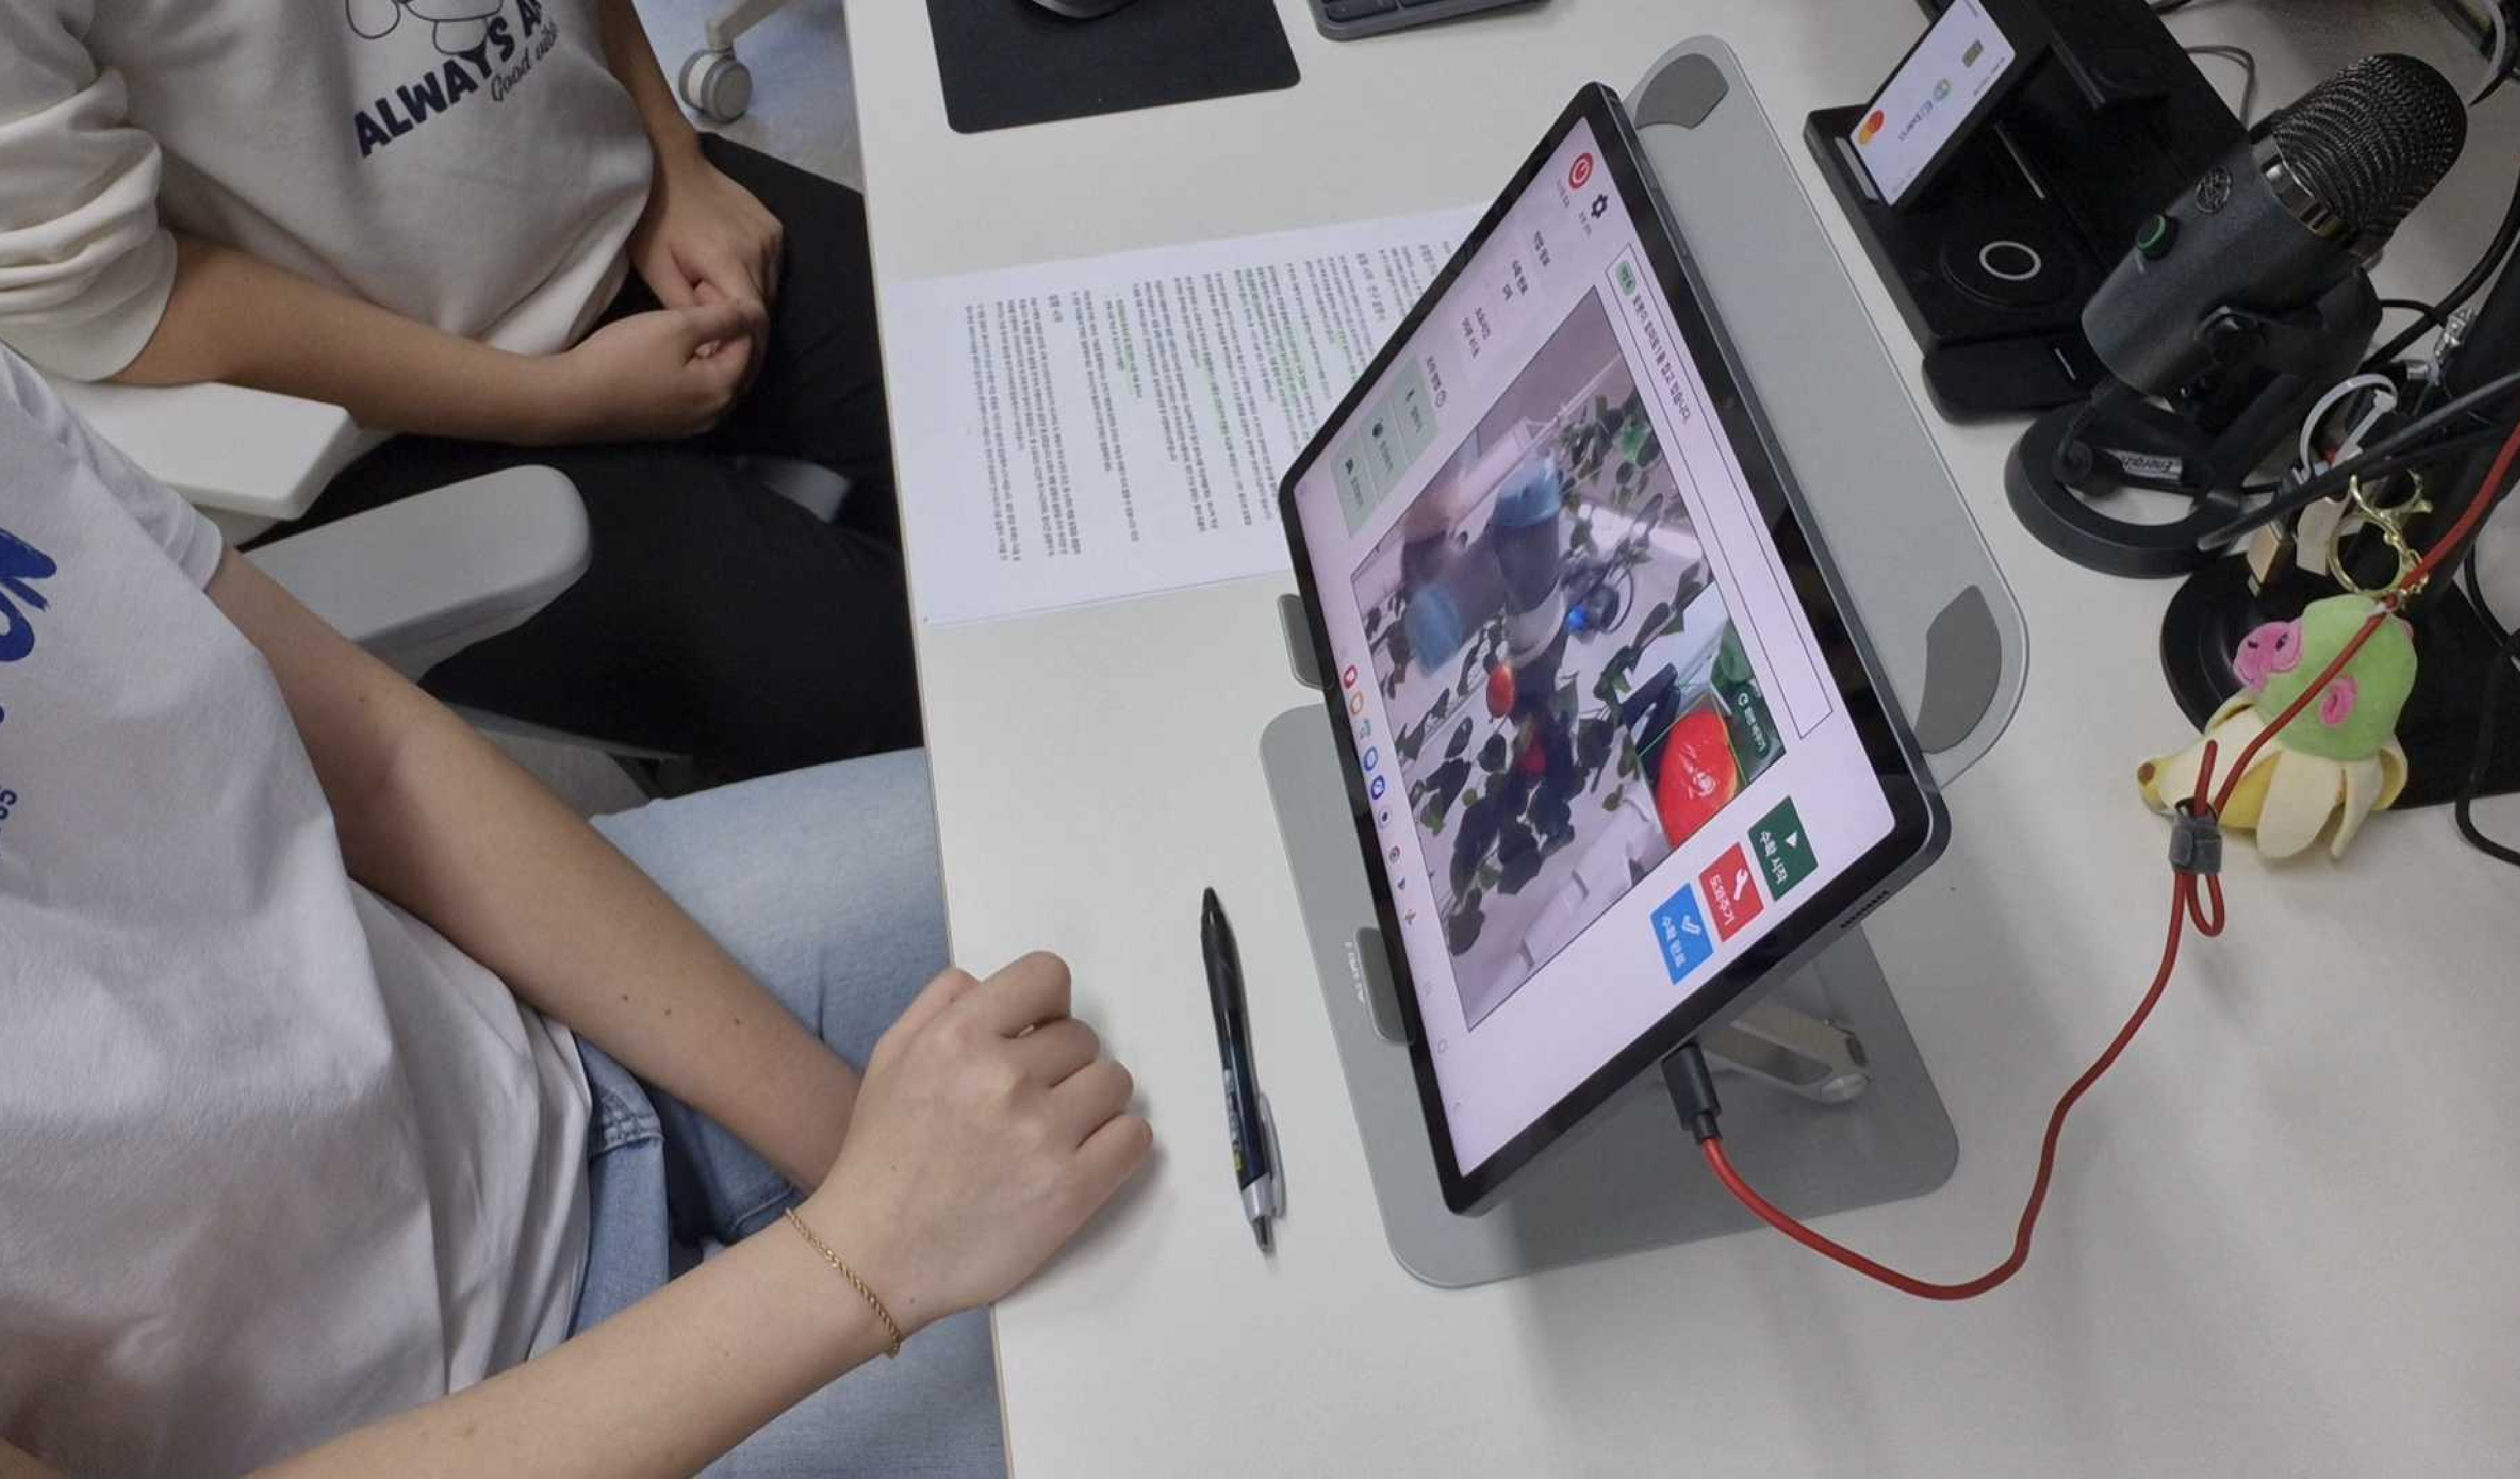
\includegraphics[width=\linewidth]{figures/10_APPX/p2_test.pdf}
\caption{P2, Harvest}
\label{fig:app_human_harvest}
\end{subfigure}
\caption{Human evaluation using the tablet interface. (a)-(b) Participants view robot camera feeds and answer queries in Sort and Harvest, respectively.}
\label{fig:app_human_tablet}
\end{figure}

\subsection{Interview Summary}\label{appx:user_interviews}
Table~\ref{tab:app_interview_summary} summarizes the five interviews discussed in Sec.~\ref{exp:interviews}.
% Excerpts are translated from Korean with speech fillers omitted. Bracketed method names replace interview labels A/B.

\begin{table}[!htbp]
\centering
\caption{Interview excerpts on baseline comparison with human response.}
\label{tab:app_interview_summary}
\small
\setlength{\tabcolsep}{5pt}
\renewcommand{\arraystretch}{1.12}
\begin{tabularx}{\textwidth}{@{}l>{\hsize=1.25\hsize\linewidth=\hsize\raggedright\arraybackslash}X>{\hsize=.75\hsize\linewidth=\hsize\raggedright\arraybackslash}X@{}}
\toprule
Participant & Interview excerpts & Interpretation \\
\midrule
% Sources: 08_Delete_Me/00_real_human/p001/p001_v2.txt, participant turns at lines 286--287 and 241--242.
P1 & ``I think errors are much less likely with [Ours].''\par For KnowNo: ``I expected it to pick the object and check its quality.'' & Links perceived reliability to fewer errors and identifies an expectation that a selected action includes preceding steps. \\
\addlinespace
% Source: 08_Delete_Me/00_real_human/p002/p002_v1.txt, participant turn at lines 476--477.
P2 & ``With [Ours], I assume the task will be completed unless I give an incorrect answer. With [KnowNo], the choices looked executable on the screen, but some did not work after I selected them.'' & Connects expected task completion with state confirmation and reports failed execution despite apparently feasible choices. \\
\addlinespace
% Source: 08_Delete_Me/00_real_human/p003/p003_v1.txt, participant turn at lines 148--149.
P3 & ``I chose the quality check because I was focused on the goal, but perhaps because I selected it before picking, it showed a failure.'' & Matches the Harvest failures involving actions selected before their preconditions are satisfied. \\
\addlinespace
% Sources: 08_Delete_Me/00_real_human/p004/p004_v1.txt, participant turns at lines 59--61 and 246--247.
P4 & For KnowNo: ``Looking back, I think I skipped a stage because I was impatient, and that seems to be why it failed.''\par For Ours: ``I only assess the state, and the robot handles most of the actions.'' & Links skipped stages to failure and describes leaving subsequent actions to the robot, supporting the division of responsibilities discussed in the main text. \\
\addlinespace
% Source: 08_Delete_Me/00_real_human/p005/p005_v1.txt, participant turn describing fact confirmation and action commands.
P5 & ``One robot asked whether something was correct; the other asked me to specify the next action.'' & Distinguishes fact verification from action decisions, consistent with the roles assigned to participants in the two methods. \\
\bottomrule
\end{tabularx}
\end{table}
